\documentclass[11pt]{article}
\usepackage{epsfig}
\usepackage{amsfonts}
\usepackage{amssymb}
\usepackage{amstext}
\usepackage{amsmath}
\usepackage{xspace}
\usepackage{theorem}
\usepackage{hyperref}
\usepackage{fullpage}
\usepackage{enumitem}
\usepackage{listings}
\usepackage{titlesec}
\usepackage{bm}
\newlist{todolist}{itemize}{2}
\setlist[todolist]{label=$\square$}
\usepackage{pifont}
\newcommand{\R}{\mathbb{R}}
\newcommand{\cmark}{\ding{51}}%
\newcommand{\xmark}{\ding{55}}%
\newcommand{\done}{\rlap{$\square$}{\raisebox{2pt}{\large\hspace{1pt}\cmark}}%
\setlength\parindent{0pt}
\hspace{-2.5pt}}
\newcommand{\wontfix}{\rlap{$\square$}{\large\hspace{1pt}\xmark}}
 \usepackage[parfill]{parskip} 
\usepackage{mathtools}
\usepackage{todonotes}
\newcommand{\comment}[1]{} 

\usepackage{graphicx}
\graphicspath{{images/}}

\newcommand{\sq}{\mathit{Q}}
\DeclarePairedDelimiter\ceil{\lceil}{\rceil}
\DeclarePairedDelimiter\floor{\lfloor   }{\rfloor}

\hypersetup{
    colorlinks   = true,
    linkcolor    = magenta
}

\newcommand{\ra}{\rightarrow}

\title{Technical Summary: ``An Improved Data Stream Summary: The Count-Min Sketch and its Applications'' 
by Cormode and Muthukrishnan}
\author{Ravi Gaddipati, Matthew Ige, and Emily Wagner}
\begin{document}
\maketitle
\section{Problem Statement and Overview}
Consider a vector $\vec{a}(t) = [a_1(t), \dots, a_i(t), \dots a_n(t)]$ which evolves with time.
Initally, $\vec{a}$ is the zero vector $\vec{0}$.  We represent the $t$th update as $(i_t, c_t)$,
which modifies the vector as follows:
\begin{align}
    a_{i_t}(t) = a_{i_t}(t - 1) + c_t, \\
    a_{i'}(t) = a_{i'}(t - 1), \, i' \neq i_t
\end{align}
The update $(i_t, c_t)$ modifies the $i$th element by adding $c_t$ to it.
For all other $a_{i'}$, the vector remains unchanged. 

This vector and its updates represent some stream of data that evolves with
time. There are 2 main models for such a stream:
\begin{enumerate}
    \item \textbf{cash-register case:} $c_t > 0$, so every vector element is monotonically
    increasing.
    \item \textbf{turnstile case:} $c_t$ can also be negative.  There are two subcases:
    \begin{enumerate}
        \item \textbf{non-negative turnstile:} $(i_t, c_t)$ will never cause vector elements
        $a_{i_t}$ to dip below zero. This guarantee can be provided by the application.
        \item \textbf{general turnstile:} vector elements $a_{i_t}$ may become negative.
    \end{enumerate}
\end{enumerate}

The basic problem this work addresses is to summarize or calculate certain
characteristics about the stream. There are 2 main constraints. First, the space
used by such algorithms should be small; at most polylogarithmic in $n$.  This
compressed version of the data is called a \textbf{sketch}.  Second, updates to
the sketch should be processed quickly.  

Since we are sublinear in input space, we will have to approximate almost any
function we want to compute over $\vec{a}$, but we still want to specify an
approximation parameter $\varepsilon$ and bound the probability of error by
$\delta$.  

The \textbf{count-min sketch} addresses these requirements and allows us to calculate several characteristics
of a stream using a single type of data structure.  It can be used to approximate three types of \textbf{queries}:
\begin{enumerate}
    \item \textbf{point query:} $\sq(i)$ is an approximation of the vector 
    element $a_i(t)$
    \item \textbf{inner product query:} $\sq(\vec{a}, \vec{b})$ approximates
    $\vec{a} \odot \vec{b} = \sum_{i = 1}^{n} a_i b_i$
    \item \textbf{range query:} $\sq(l, r)$ is an approximation of 
    $\sum_{i = l}^{r}a_i$. 
\end{enumerate}

These queries can be used for more complex data stream functions, such as $\phi$-quantiles and heavy hitters,
which will be described in section \ref{sec:applications}.

\section{State of the art}
Sketches have been commonly used to help analyze large streams of data. \comment{These sketches allow for the following types of queries: $L_1$ and $L_2$ norms, number of distinct items in a sequence, join size of relations, range sum queries, and more.} Although these data structures have proved to be very powerful, there are a few key drawbacks that limit the effectiveness of these sketches:
\begin{enumerate}
    \item Common sketches (\cite{AGMS99}, \cite{CCF02}, \cite{GKMS02})  typically use $\Omega(\frac{1}{\varepsilon^2})$ space. For common uses of $\varepsilon$, like 0.1 or 0.01, this scaling can quickly become too expensive.
    \item Many sketches take linear time (in the size of the sketch) to do a single update(\cite{AGMS99}, \cite{GKMS02}).
    \item Some sketches require $4$-wise independent hash functions \cite{AGMS99}. This is not trivial, and is especially difficult in hardware applications.
    \item Some sketches can only handle one particular query.
    \item Many sketches use analysis that hides large constants (\cite{CCF02}).
\end{enumerate}
The count-min sketch reduces these problems in the following ways:
\begin{enumerate}
    \item CMS uses space proportional to $\frac{1}{\varepsilon}$.
    \item Update time is sublinear with respect to the size of the sketch.
    \item CMS requires only pairwise independent hash functions.
    \item The sketch can answer several queries and has numerous applications.
    \item All constants are explicit and small.
\end{enumerate}
In particular, notice that the space has been reduced from
$\frac{1}{\varepsilon^2}$ to $\frac{1}{\varepsilon}$ using a CMS, and the time
for an update has been reduced from $\frac{1}{\varepsilon^2}\ln{\frac{1}{\delta}}$
to $\ln{\frac{1}{\delta}}$ (count sketch also has this update time, however).

\section{How to make a count-min sketch}
Note $e$ is the base of the natural logarithm function, $\ln$. The count-min
sketch is an array with $w$ columns and $d$ rows where:
\begin{align}
    w = \ceil{e/\varepsilon}\\
    d = \ceil{\ln{1/\delta}}
\end{align}
for a given accuracy parameter $\varepsilon$ and probability guarantee $\delta$.
We need $d$ pair-wise independent hash functions
\begin{align}
    h_1 \dots h_d : \{1 \dots n\} \ra \{1 \dots w\} 
\end{align}
The sketch starts with every array entry being 0. The count-min sketch $count$
is updated when the $t$th update $\{a_{i_t}, c_t\}$ arrives as follows
\begin{align}
    count[j, h_j(i_t)] \leftarrow count[j, h_j(i_t)] + c_t     
\end{align}
In other words, upon receiving an update $(i_t, c_t)$:
\begin{lstlisting}[escapeinside={(*}{*)}]
Update_CM_Sketch(count, (*$(i_t, c_t)$*)) 
    for each row j, 1 (*$\leq$*) j (*$\leq$*) d:
        count[j, (*$h_j(i)$*)] (*$\leftarrow$*) count[j, (*$h_j(i)$*)] + (*$c_t$*)
    return count 
\end{lstlisting}

\comment{
\begin{enumerate}
    \item for each row $1 \leq j \leq d$
    \begin{enumerate}
        \item add $c_t$ to the $h_j(i)$th column.
    \end{enumerate}
\end{enumerate}
}


\section{Approximate Point Queries using CM sketches}

\subsection{Non-Negative Case}
\subsubsection{Algorithm}
For the non-negative case (either the non-negative turnstile or cash-register case),
the algorithm to estimate $\hat{a}_i(t) = \sq(i)$ is as follows: 
\begin{align}
    \sq(i) = \hat{a}_i = \text{min}_j count[j, h_j(i)]
\end{align}
In other words for a given $\hat a_i(t) =$ \texttt{Estimate\_Point\_Query(count, $i_t$)}.

\begin{lstlisting}[escapeinside={(*}{*)}]
Estimate_Point_Query(count, (*$i_t$*)) 
    s (*$\leftarrow$*) (*$\infty$*)
    for each row j, 1 (*$\leq$*) j (*$\leq$*) d:
        if count[j, (*$h_j(i)$*)] < s:
            s (*$\leftarrow$*) count[j, (*$h_j$*)(i)]
    return s;
\end{lstlisting}

\textbf{Theorem 1:} The estimate $\hat a_i$ has the following guarantees:
\begin{enumerate}[label=\textnormal{(\arabic*)}]
    \item $a_i \leq \hat{a}_i$
    \item with probability at least $1 - \delta$, $\hat{a}_i \leq a_i + \varepsilon ||\vec{a}||_1$
\end{enumerate}
\subsubsection{Proof of Theorem 1}
First, we prove 1.a.  

\textbf{Define} an indicator variable $I_{i, j, k}$ as follows:
\begin{align}
    I_{i, j, k} = 
    \begin{cases}
        1, & \text{ if } h_j(i) = h_j(k) \text{ and } i \neq k \\
        0, & \text{otherwise}
    \end{cases}
\end{align}
$I_{i, j, k}$ is 1 if $i$ and $k$, $i \neq k$, have a collision under hash function $h_j$.

Since, to begin with, we chose all $h_j$ from a 2-universal hash family
with range $1 \leq h_j \leq d = \ceil{\frac{e}{\varepsilon}}$ 
we know that, for $i \neq k$,
\begin{align}\label{eq:collision-prob}
    &Pr(h_j(i) = h_j(k)) \leq \frac{1}{\text{range}(h_j)} = 1/\ceil{\frac{e}{\varepsilon}} = \floor{\frac{\varepsilon}{e}} \nonumber\\
    \implies &E(I_{i, j, k}) \leq \frac{\varepsilon}{e}
\end{align}
by the properties of a 2-universal hash function and by our choice of hash function
range.

\textbf{Define} $X_{i, j}$ as follows:
\begin{align}
    X_{i, j} = \sum_{k = 1}^{n}I_{i, j, k} a_k
\end{align}
In other words, $X_{i, j}$ is the sum of all corresponding vector values whose indices
$i$ collide under $h_j$. Trivially, we can then state that
\begin{align}\label{eq:count-def}
    count[j, h_j(i)] = a_i + X_{i, j} 
\end{align}
Now, Theorem 1.a follows because we are only considering the case where vector
elements are non-negative and thus
\begin{align}
    a_i \leq \hat a_i = a_i + X_{i, j}
\end{align}

Now we show 1.b.

For future use in the analysis, we evaluate:
\begin{align}
    E(X_{i, j}) = E\left(\sum_{k = 1}^n I_{i, j, k} a_k\right) 
\end{align}
by definition of $X_{i, j}$. The linearity of expectation states that
\begin{align}
    E(\sum_{i = 1}^{n} c_i X_i) = \sum_{i = 1}^{n} c_i E(X_i)
\end{align}
where $X_i$s may be dependent. Applying linearity of expectations here, we have:
\begin{align}
    E(\sum_{k = 1}^{n} a_k I_{i, j, k}) = \sum_{k = 1}^{n} a_k E(I_{i, j, k}) 
\end{align}
% why less than equals, why not just equals?
We showed $E(I_{i, j, k}) \leq \frac{\varepsilon}{e}$ in Equation \ref{eq:collision-prob}, so 
we have
\begin{align}
    \sum_{k = 1}^{n} a_k E(I_{i, j, k})  \leq\sum_{k = 1}^{n} a_k \frac{\varepsilon}{e}
\end{align}
and finally, since $||\vec{a}||_1 = \sum_{k = 1}^{n} |a_k| = \sum_{k = 1}^{n} a_k$
(all $a_k$ are assumed to be non-negative)
\begin{align}\label{eqn:expectation-bound}
    \sum_{k = 1}^{n} a_k \frac{\varepsilon}{e} = \frac{\varepsilon}{e} ||\vec{a}|||_1 \nonumber \\
    \implies E(X_{i, j}) \leq \frac{\varepsilon}{e} ||\vec{a}||_1 
\end{align}
We will use this result in the following proof.

We want to show that $Pr[\hat{a}_i > a_i + \varepsilon ||a||_1] < \delta$. We can see that
\begin{align}
    Pr[\hat{a}_i > a_i + \varepsilon ||a||_1] = Pr[\forall_{j \cdot} count[j, h_j(i)] > a_i + \varepsilon ||\vec{a}||_1 ]
\end{align}
since the probability that all values in a set are greater than $a_i + \varepsilon||\vec a||_1$ is equivalent 
to the probability that the minimum of all the values in that set is greater than $a_i + \varepsilon||\vec a||_1$.
(Recall that $\hat a_i$ is defined as the minimum of all of the array elements that $i$
hashes to in each row.) Then, by the definition stated in equation \ref{eq:count-def}, we have
\begin{align}
    Pr[\forall_{j \cdot} count[j, h_j(i)] > a_i + \varepsilon ||\vec{a}||_1] = Pr[\forall_{j \cdot} a_i + X_{i, j} > a_i + \varepsilon ||\vec{a}||_1]
\end{align}
Then, subtracting $a_i$ from both sides, and using equation \ref{eqn:expectation-bound} on the $\varepsilon ||\vec{a}||_1$ term, we have:
\begin{align}
    Pr[\forall_{j \cdot} a_i + X_{i, j} > a_i + \varepsilon ||\vec{a}||_1] \geq Pr[\forall_{j \cdot} X_{i, j} > e E(X_{i, j})]
\end{align}

Finally, consider the Markov inequality:
\begin{align}
    Pr[X > aE[X]] \leq \frac{1}{a}
\end{align}
Since this is the non-negative case and thus $X_{i, j}$ is non-negative, we can apply it here:
\begin{align}
    Pr[X_{i, j} > e E(X_{i, j})] \leq \frac{1}{e} \\
    \implies \bigcap_{1 \leq j \leq d} Pr[X_{i, j} > e E(X_{i, j})] \leq \left(\frac{1}{e}\right)^d \\
    \implies Pr[\forall_{j \cdot} X_{i, j} > e E(X_{i, j})] \comment{\leq \frac{E(X_{i, j})}{a_i + \varepsilon||a||_1} \leq \frac{\ceil{\frac{\varepsilon}{e}} ||\vec{a}||_1}{a_i + \varepsilon||a||_1}}
      \leq e^{-d} \leq \delta
\end{align}
Note that we can use the intersection bound here because our hash functions for
each row were picked independently and uniformly at random from a 2-universal
hash-family.

This estimate is calculated in $O(\ln \frac{1}{\delta})$ as the minimum of a
multiset can be taken in linear time, and we are taking it across $d = O(\ln
\frac{1}{\delta})$ rows for the point query.  The update time to maintain the
data structure after each update is also $O(\ln \frac{1}{\delta})$, since we
hash a single value in each row of the data structure.

The space complexity is $O\left({\frac{e}{\varepsilon}}{\ln
\frac{1}{\delta}}\right)$ words, as the dimensions of the matrix are $w \times d =
\ceil{\frac{e}{\varepsilon}}\times\ceil{\ln \frac{1}{\delta}}$.  $O(\ln
\frac{1}{\delta})$ is also required to store the hash functions.  The constants
are clearly small, since this is the total space requirement.

All previous analyses of sketch algorithms use Chebyshev in their estimation analysis, yielding a dependency on
$\frac{1}{\varepsilon^2}$ for the space complexity.  Using Markov in this analysis yields a tighter bound,
with a dependency $\frac{1}{\varepsilon}$.

\subsection{General Case}
\subsubsection{Algorithm}
The algorithm is identical to the non-negative case, except that we take the median among the rows:
\begin{align}
    \sq(i) = \hat{a}_i = \text{median}_j count[j, h_j(i)]
\end{align}

\textbf{Theorem 2:} With probability $1 - \delta^{1/4}$,
\begin{align}
    a_i - 3\varepsilon||\vec{a}||_1 \leq \hat{a}_i \leq a_i + 3\varepsilon||\vec{a}||_1. 
\end{align}
Here, since the array elements can be negative, we can no longer use Markov, and instead must apply Chernoff
bounds. 

The time and space complexity are the same as the non-negative case: $O(\ln
\frac{1}{\delta})$ time and $O(\frac{e}{\varepsilon}\ln \frac{1}{\delta})$
words, respectively. {

\section{Inner Product Query}
	\subsection{Algorithm: Non-negative case}
        Two CM sketches are kept, one for vector $a$ and one for vector $b$.
        Updates to each sketch take the form $(i_t,c_t)_v: count_v(j, h_j[i]) \leftarrow
        count_v(j, h_j[i]) + c_t$. To compute the estimated inner product
        $\widehat{\vec{a} \odot \vec{b}}$, we compute the inner product of each
        row pair $count_a[j] \cdot count_b[j]$ for all $j \in d$, taking the
        minimum. Formally, the estimate for the inner product
        $\mathit{Q}(\vec{a},\vec{b})$ for non-negative vectors $\vec{a}$ and
        $\vec{b}$ is $\widehat{\vec{a} \odot \vec{b}} = \min_j(\widehat{\vec a
        \cdot \vec b})_j$, where $(\widehat{\vec a \cdot \vec b})_j =
        \sum_{k=1}^w count_a[j,k] * count_b[j,k]$. In psuedocode form:\\
        
\begin{lstlisting}[escapeinside={(*}{*)}]
Estimate_Inner_Product((*$count_a, count_b$*)): 
    make empty set Estimates 
    for each row j, 1 (*$\leq$*) j (*$\leq$*) d:
        Estimates[j] (*$\leftarrow$*) (*$\sum_{k=1}^w$*) (*$count_a[j, k] * count_b[j,k]$*)
    return min(Estimates) 
\end{lstlisting}
\textbf{Theorem 3:}\\
        The estimate $\widehat{\vec{a} \odot \vec{b}}$ has the following guarantees:
        \begin{enumerate}[label=\textnormal{(\arabic*)}]
            \item $\vec a \odot \vec b \leq \widehat{\vec a \odot \vec b}$
            \item with probability at least $1 - \delta$, 
            \begin{align}
		        Pr(\widehat{\vec a \odot \vec b} \leq \vec a \odot \vec b + \varepsilon||\vec a||_1||\vec b||_1)
            \end{align}
        \end{enumerate}
	\subsection{Proof of Theorem 3}
		We represent the estimated inner product as the sum of the true inner product and collisions. By the pairwise independence of all hash functions $h_j$, $1 \leq j \leq d$,
		\begin{align}
		(\widehat{\vec a \cdot \vec b})_j &= \sum_{i=1}^n a_ib_i + \sum_{p \neq q, \,\,\ h_j(p)=h_j(q)} a_pb_q
        \end{align}
        Taking the expected value of the error term shows that the error is dependent on the probability of collision.
        \begin{align}
		E\left[(\widehat{\vec a \cdot \vec b})_j - \vec a \cdot \vec b\right] &= E\left[\sum_{p \neq q, \,\, h_j(p)=h_j(q)} a_pb_q\right] \\
		&= \sum_{p \neq q}Pr(h_j(p) = h_j(q))a_pb_q
        \end{align}

        Using the results from Theorem 1, we know the probability of collision is bounded by $\varepsilon/\mathrm e$ where $\varepsilon$ is the parameter used during sketch construction.
        \begin{align}
		&\leq \sum_{p \neq q} \frac{\varepsilon}{\mathrm{e}}a_pb_q \\
		E\left[(\widehat{\vec a \cdot \vec b})_j - \vec a \cdot \vec b\right]&\leq \frac{\varepsilon}{\mathrm e}||a||_1||b||_1
		\end{align}
		This follows by the treatment of the inner product computation as a series of point queries. Applying the Markov inequality we bound the probability of the error.
		\begin{align}
		Pr((\widehat{a \cdot b})_j - \vec a \cdot \vec b > \varepsilon ||a||_1||b||_1) &\leq \frac{E[\widehat{a \cdot b} - a \cdot b]}{\varepsilon||a||_1||b||_1} \\
		&\leq \frac{\frac{\varepsilon}{\mathrm e}||a||_1||b||_1}{\varepsilon||a||_1||b||_1} \\
		& \leq 1/e
        \end{align}
        As defined in the construction of the CM sketch, $d = \ln 1/\delta$, so
        $\delta = e^{-d}$. The probability the error exceeds this threshold for
        a single estimator is less than or equal to $1/e$ as shown above. Since we take the
        minimum inner product as our estimate, we compute the probability all
        estimators exceed this threshold.
        \begin{align}
        \bigcap_{1\leq j \leq d} Pr((\widehat{\vec a \cdot \vec b})_j - \vec a \cdot \vec b > \varepsilon ||a||_1||b||_1) &\leq \left(\frac{1}{\mathrm e}\right)^d \\
        &\leq \delta
        \end{align}
        for all $d > 0$.


\section{Range Query: Non-negative}
A range query, denoted as: $\mathcal{Q}(l,r)$, requests the value:
\begin{align*}
    a[l,r] = \sum_{i=l}^r a_i
\end{align*}
And we denote our estimator based on the CM sketch as: $\hat a[l,r]$. It is
possible to simply query all values in the range, $\hat a[l,r] = \sum_{i=l}^r
\hat a_i$, however, this query would take linear time with respect to the input.
Additionally, our error bound would have an extra multiplicative term in the
length of the range, $r - l$. We can utilize dyadic ranges to help address both
of these issues.
\subsection{Dyadic ranges}
For any range, we can create a set of dyadic ranges by splitting the range in
half to get two ranges of half the size. We can continually do this, until we
have ranges of size 1. We can think of the construction of a set of dyadic
ranges as creating a tree-like structure:
\begin{center}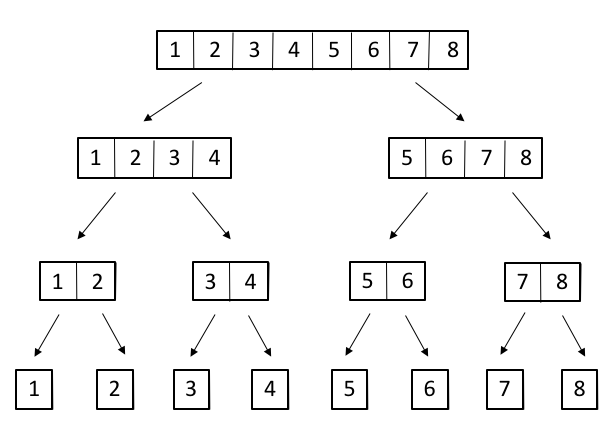
\includegraphics[scale=0.3]{dyadic_ranges.png}\end{center}
\subsection{Range Query: updates}
The update procedure is as follows: Keep $\log_2n$ CM sketches. Each CM sketch
represents one level of our ``tree'' of dyadic ranges, and the keys for that CM
sketch are the ranges within that level, and the values are the sum of the counts for all
values in the range of each key:
\begin{center}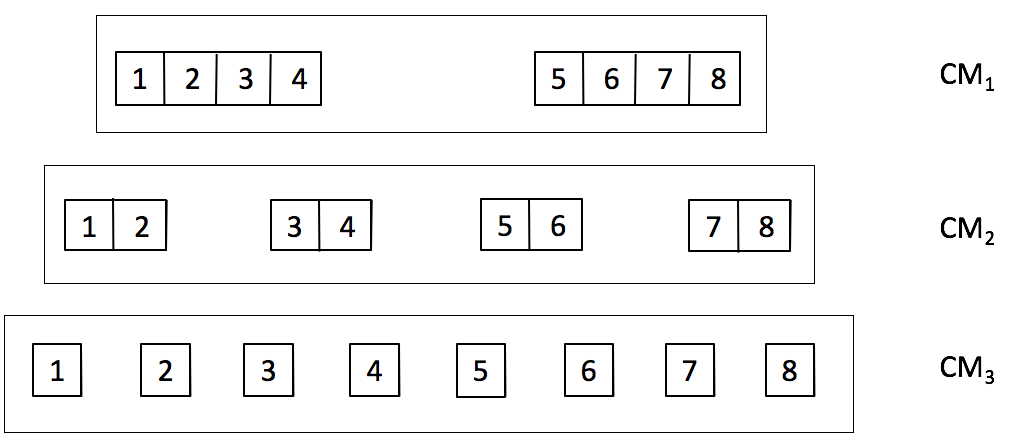
\includegraphics[scale=0.3]{dyadic_ranges_cm.png}\end{center}
When we get an update, $(i_t, c_t)$, we simply update each CM sketch, with the
key as the range that covers the value $i_t$:
\begin{center}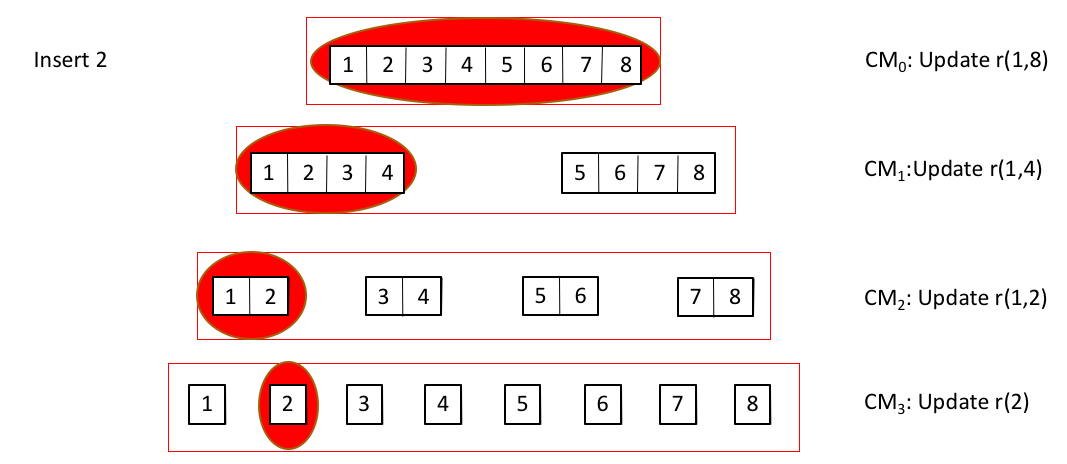
\includegraphics[scale=0.3]{range_update.png}\end{center}
We thus have the following pseudocode for an update, where \texttt{counts} is
all of the CM sketches in the tree, and $range_i(i_t)$ represents the dyadic
range that contains $i_t$, for level $i$:
\begin{lstlisting}[escapeinside={(*}{*)}]
Range_Query_Update(counts, ((*$i_t, c_t$*)))
    for each sketch, (*$count_i \in$*) counts:
        Update_CM_Sketch((*$ count_i $*), ((*$range_i(i_t$*)), (*$c_t$*)))
    return counts;
\end{lstlisting}
\subsection{Range Query: estimation}
Then, in order to estimate a range query, $\hat a[l,r]$, we identify which
dyadic ranges contribute to our overall range, and query those in each
appropriate CM sketch.
\begin{center}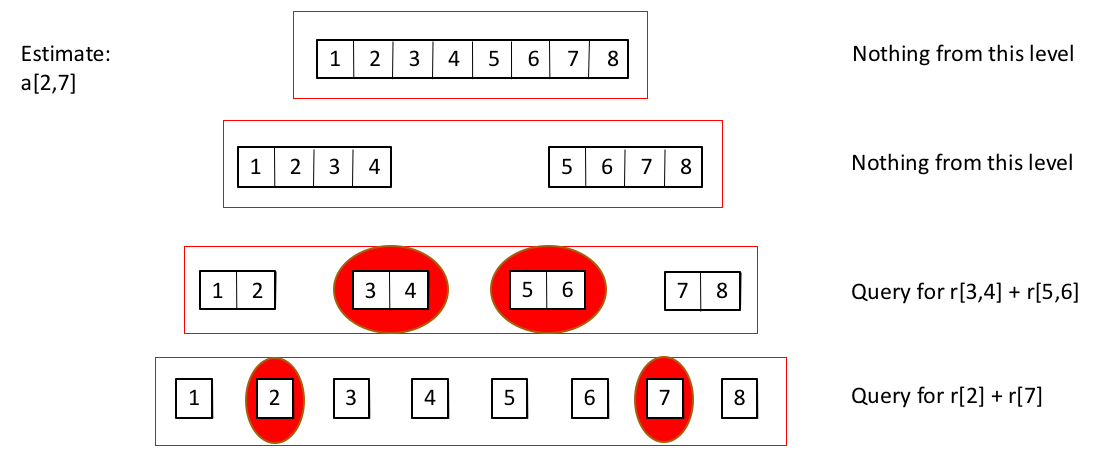
\includegraphics[scale=0.3]{range_estimate.png}\end{center}
A single range can be converted into at most $2\log_2n$ dyadic ranges, because
in the worst case, both sides of the range query (the upper bound $r$ and lower
bound $l$)  must fully travel through the height of the tree. Because we store
each dyadic range as a key value in a CM sketch, we do a total of, at most,
$2\log_2n$ point queries. We then sum together the point queries, to get our
total range query estimate. In pseudocode form, the procedure for estimation is
as follows:
\begin{lstlisting}[escapeinside={(*}{*)}]
Estimate_Range_Query(counts, a[l,r], i, x, y) 
    if (*$range(x,y) \in [l,r]$*):
        return Estimate_Point_Query((*$count_i$*), range(x,y))
    else:
        return Estimate_Range_Query(counts, a[l,r], (*$i+1, x, \frac{x+y}{2}$*)) +
            Estimate_Range_Query(counts, a[l,r], (*$i+1, \frac{x+y}{2} + 1, y$*))
\end{lstlisting}
Where $i$ denotes the level that we are looking at in our tree of dyadic ranges,
$count_i$ represents the CM sketch of that level, and each recursive call simply
alters the range we are looking for, along with going down one level in our
tree.\\\\
Finally, recall the idea behind using dyadic ranges: to reduce the estimation
time to be polylogarithmic in the size of the input. A single point query
update/estimation takes $\log(\frac{1}{\delta})$ time. In order to do a single
update, we update $O(\log n)$ CM sketches. When we estimate our range query, we
do $O(\log n)$ point query estimations. Thus, for both an update and an
    estimation, our time is reduced to $O(\log(n)\log(\frac{1}{\delta}))$.
\subsection{Theorem 4: }
\begin{enumerate}[label=\textnormal{(\arabic*)}]
    \item $a[l,r] \leq \hat a[l,r]$.
    \item With probability at least $(1-\delta)$, $\hat a[l,r] \leq a[l,r] + 2\varepsilon \log n ||\vec{a}||_1$
\end{enumerate}
    \textbf{Proof:}\\
Our procedure for estimation covers exactly the range [l,r]. We are summing up multiple point queries, and thus, based on the previous proof, (1) holds. In order to show (2), the following notation will be used:
\begin{align*}
    range[l,r] &= \text{The range from l through r}\\
    range_i &= \text{A dyadic range.}\\
    \bigcup_{range_i \in range[l,r]} range_i &= \text{A set of non-overlapping dyadic ranges that exactly cover range[l,r]}\\
\end{align*}
Thus, we show:
\begin{align*}
    \hat a[l,r] &= \sum_{range_i \in range[l,r]} a_{range_i} + \sum_{i \neq k, h_j(range_i) = h_j(range_k)} a_{range_i}\\
    E[\hat a_j[l,r] - a[l,r]] &= E[\sum_{range_i \in range[l,r]} a_{range_i} + \sum_{i \neq k, h_j(range_i)=h_j(range_k)} a_{range_i} - \sum_{range_i \in range[l,r]} a_{range_i}]\\
    &= E[\sum_{i \neq k, h_j(i)=h_j(k)} a_{range_i}]\\
    &\leq 2\frac{\varepsilon}{\mathrm e} \log n ||a||_1
\end{align*}
Where the error for a single point query is $\frac{\varepsilon}{\mathrm
e}||a||_1$, and we do at most $2log_2n$ point queries. Thus, the error is
bounded as above. We can then use the Markov inequality to bound the error
probability:
\begin{align*}
    p(\hat a_j[l,r] - a[l,r] > 2\varepsilon \log n ||a||_1) &\leq \frac{E[\hat a_j[l,r] - a[l,r]]}{2\varepsilon \log n||a||_1}\\
    &\leq \frac{2\frac{\varepsilon}{\mathrm e}\log n ||a||_1}{2\varepsilon \log n ||a||_1}\\
    &\leq \frac{1}{\mathrm e}
\end{align*}
However, this is the error bound for a single estimator. Our CM sketch construction uses d rows, and thus, to bound the error, we need to find the probability that all of our estimators exceed the threshold:
\begin{align*}
    \bigcap_{1\leq j \leq d} Pr(\hat a_j[l,r] - a[l,r] > 2\varepsilon \lg n ||\vec{a}||_1) &\leq \left(\frac{1}{\mathrm e}\right)^d = (\mathrm e)^{-d}\\
    &\leq \delta
\end{align*}
Therefore, with probability at least $(1-\delta)$, $\hat a[l,r] \leq a[l,r] + 2\varepsilon \log n ||\vec{a}||_1$
\section{Applications}\label{sec:applications}
\subsection{Quantiles in the turnstile model}
Define the $\phi$-quantiles of the cardinality
\begin{align}
    ||\vec{a}||_1 = \sum_{i = 1}^{n}|a_i(t)|
\end{align}
as the values within a multiset of finite size that split it into $\phi$ groups
of equal size based on their rank $R$.  For example, the median of a set of data
is the 2-quantile. 

To obtain the $\phi$-quantiles, the elements are sorted and split as follows.
The $k$th quantile is the element(s) with rank $R = k\phi||\vec{a}||_1$ for $k =
1, 2, \dots, 1/\phi$.  The $\varepsilon$-approximation for the $\phi$-quantiles
accepts as the $k$-th quantile any of the  values with rank $(k\phi -
\varepsilon)||\vec{a}||_1 \leq R \leq (k\phi + \varepsilon)||\vec{a}||_1$ for a
given $\varepsilon < \phi$.


The count-min sketch can be used to calculate the $\phi$-quantiles in the turnstile model.
In this case, updates where $c_t < 0$ are called deletions, and $c_t > 0$ are called insertions.
The value for each vector element $a_i$ is actually the number of instances of the element
$i$.

Prior work \cite{GKMS02} shows that $\phi$-quantiles in this model can be approximated using range sums. This is done
as follows:
\begin{enumerate}
    \item For each $k \in {1, 2, \dots, 1/\phi}$
    \begin{enumerate}
        \item Find a range sum such that $a[1, r]$ is the $\varepsilon$-approximation for $k\phi||\vec{a}||_1$. Find $r$ using a binary
        search on the possible range sums $a[1, \hat{r}]$, where $\hat{r} \in \{1, 2, \dots, n\}$.  $r$ is the
        $\varepsilon$-approximation for the $k$th $\phi$-quantile.
    \end{enumerate}
\end{enumerate}
The method in \cite{GKMS02} uses Random Subset Sums to approximate range sums.  If instead a count-min
sketch is used to approximate the range sums, better results follow.  

To use a count-min sketch to approximate quantiles in the turnstile model, $\log n$ sketches are kept,
one for each dyadic range. Each sketch gets accuracy parameter $\varepsilon/\log n$ for an overall accuracy
bounded by $\varepsilon$. Each sketch gets probability guarantee $\delta\phi/\log n$, for
an overall probability guarantee of $\delta$ for all $1/\phi$ quantiles. Then, we have the following:

\textbf{Theorem 5:} $\varepsilon$-approximate $\phi$-quantiles can be found with probability at least
$1 - \delta$ by keeping a data structure with space $O\left(\frac{1}{\varepsilon}
\log^2(n) \log \left(\frac{\log n}{\phi \delta}\right)\right)$ The time for each insert or delete operation is
$O\left(\log(n) \log \left(\frac{\log n}{\phi \delta}\right)\right)$, and the time to find each quantile on demand 
is $O\left(\log(n)\log\left(\frac{\log n}{\phi \delta}\right)\right)$

This improves the existing query time and update by a factor of more than $\frac{34}{\varepsilon^2} \log n$
The space requirements are improved by a factor of at least $\frac{34}{\varepsilon}$. 

\subsection{Heavy Hitters}
A potential application of the count min sketch is the heavy hitters problem. Given an input $A$ of length $n$ and a parameter $k$ we wish to return values that occur in the input at least $n/k$ times. There may be at most $k$ such heavy hitters, though there also may be none. This sketch provides a convenient way to find the heavy hitters of some data stream with a large input size for which  maintaining a counter for each unique element is not feasible. We look at two cases:
\begin{enumerate}
\item The cash register case: elements are only added
\item The turnstile case: elements can be added or removed
\end{enumerate}

\subsubsection{Cash Register Case}
\textbf{Algorithm:}\\
We can easily obtain $||\vec{a}||_1$ at any given point in time because it is
simply: $\Sigma_{i=1}^t c_i$.We define a $\phi$ heavy hitter if the estimation
of the point query, $Q(i_t) =  \hat a_{it} \geq \phi ||\vec{a}(t))||_1$. We can
do this by maintaining a heap to store the items above the
$\phi||\vec{a}(t)||_1$ threshold. On any update, we check the lowest value
in the heap, and if the update would be greater than the lowest item, we
replace it in the heap. When we are finished with the stream, we do a final
scan of all items in the heap, and return the ones which have a value over
$\phi||\vec{a}||_1$.

\textbf{Theorem 6: } We can identify the heavy hitters of a sequence of length
$||\vec{a}||_1$ using space
$O(\frac{1}{\varepsilon}log(\frac{||\vec{a}||}{\delta}))$ and time
$O(log(\frac{||\vec{a}||}{\delta}))$. Every item which occurs with count at
least $\phi ||\vec{a}||_1$ is output, and with probability $(1-\delta)$, no
items whose count is less than $(\phi - \varepsilon)||\vec{a}||_1$ are output.

\textbf{Proof idea:}\\
Because we have only positive updates, and a CM sketch will only over estimate
any $a_i$, it is not possible to miss any heavy hitter.  In order to calculate
the error bound, we simply scale the parameter, $\delta$, such that the
probability of erroring at any point throughout the stream is bounded by
$(1-\delta)$. This requires using the union bound for time $t$,
and solving for the appropriate $\delta$.

\subsubsection{Turnstile Case}
\textbf{Algorithm:}\\
The method outlined by Graham Cormode et. al. \cite{CM03} is adapted using the count min
sketch. In this scheme, a sketch is maintained for each of the $\log n$ dyadic
ranges. These sketches are kept in a binary tree. When an update $(i_t, c_t)$ is
received, a tree search for $a_i$ is performed. As the tree is traversed, the CM
sketch at each level is updated to reflect $(i_t, c_t)$. To find the heavy
hitters, a binary search is performed recursively searching each range for which
the counter weight exceeds $(\phi + \varepsilon)||a||_1$.

\textbf{Theorem 7:} \\
The algorithm uses space $O((1/\varepsilon)\log n \log (2 \log n/(\delta
\phi)))$ and time $O(\log n \times \log(2 \log n/(\delta\phi)))$ per update.
Every item with frequency at least $(\phi + \varepsilon)||a||_1$ is reported,
and with probability $1-\delta$ no item whose frequency is less than $\phi
||a||_1$ is output.\\ 
\textbf{Proof idea:}\\
Since at each level there are at most $1/\phi$ items with frequency greater than
$\phi$, the probability of failure for each sketch is set at $\delta\phi/(2\log
n)$ to limit the number of output items whose true frequency is less than
$\phi$. By doing this the total probability that there is any overestimated by
more than $\varepsilon$ is bounded by $\delta$ by the union bound.  Since the
sketch at minimum reports the true count, we are guaranteed that the the true
heavy hitters, if they exist, are reported. With probability $\delta$, the
algorithm will report a false heavy hitter.

\bibliographystyle{plain}
\bibliography{count_min_sketch}{}
\end{document}

